% flashcards-title: Two candidate system boundaries
% flashcards-desc: A book stands on a table. To the right, two shelf boards form an open gap. Dashed loop A encloses only the book; a larger dashed loop B encloses the book, the space between, and the shelf gap.
\documentclass[dvisvgm,tikz,border=8pt]{standalone}
\usepackage{tikz}
\usetikzlibrary{arrows.meta,calc,positioning}
\definecolor{DeckInk}{HTML}{172A3A}
\definecolor{DeckAccent}{HTML}{176B87}
\definecolor{DeckWarm}{HTML}{D97706}
\definecolor{DeckMuted}{HTML}{667784}
\definecolor{DeckPaper}{HTML}{F7FAFC}
\tikzset{
  every node/.style={font=\sffamily, text=DeckInk},
  object/.style={draw=DeckInk, line width=1.1pt, fill=DeckPaper},
  primary/.style={draw=DeckAccent, line width=1.5pt},
  boundary/.style={draw=DeckAccent, line width=1.5pt, dashed, rounded corners=6pt},
  guide/.style={draw=DeckMuted, line width=0.9pt, dashed},
  dimension/.style={{Stealth[length=3.2mm,width=2.2mm]}-{Stealth[length=3.2mm,width=2.2mm]}, draw=DeckWarm, line width=1.2pt},
  motion/.style={-{Stealth[length=3.5mm,width=2.5mm]}, draw=DeckAccent, line width=1.5pt, dashed},
}

\begin{document}
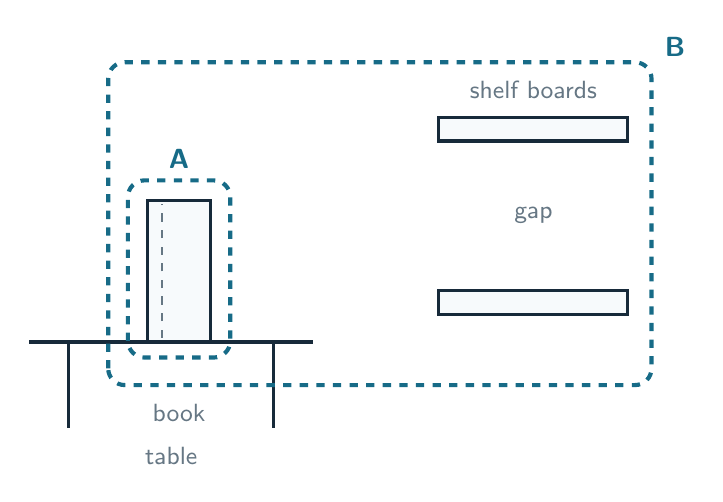
\begin{tikzpicture}[x=1cm,y=1cm]
  % Table: top surface and two legs
  \draw[object, fill=none, line width=1.3pt] (-0.4,0) -- (3.2,0);
  \draw[object, fill=none] (0.1,0) -- (0.1,-1.1);
  \draw[object, fill=none] (2.7,0) -- (2.7,-1.1);
  \node[text=DeckMuted, font=\sffamily\small] at (1.4,-1.45) {table};

  % Book standing on the table
  \draw[object] (1.1,0) rectangle (1.9,1.8);
  \draw[guide] (1.28,0.05) -- (1.28,1.75);
  \node[text=DeckMuted, font=\sffamily\small] at (1.5,-0.9) {book};

  % Shelf boards forming an open gap
  \draw[object] (4.8,0.35) rectangle (7.2,0.65);
  \draw[object] (4.8,2.55) rectangle (7.2,2.85);
  \node[text=DeckMuted, font=\sffamily\small, align=center] at (6.0,3.2) {shelf boards};
  \node[text=DeckMuted, font=\sffamily\small] at (6.0,1.6) {gap};

  % Candidate boundary A: book only
  \draw[boundary] (0.85,-0.2) rectangle (2.15,2.05);
  \node[text=DeckAccent, font=\sffamily\bfseries] at (1.5,2.32) {A};

  % Candidate boundary B: book plus shelf gap
  \draw[boundary] (0.6,-0.55) rectangle (7.5,3.55);
  \node[text=DeckAccent, font=\sffamily\bfseries] at (7.8,3.75) {B};
\end{tikzpicture}
\end{document}
